\documentclass{beamer}
\usetheme{metropolis}
\usepackage{graphicx}
\usepackage{subfig}
\title{Algebra-Based Physics-1: Mechanics (PHYS135A-01): Example Problems File}
\date{September 6th - September 8th, 2017}
\author{Jordan Hanson}
\institute{Whittier College Department of Physics and Astronomy}

\begin{document}
\maketitle

\section{Chapter 6}

\begin{frame}{Examples from Chapter 6}
\textbf{Conceptual Question 2.} \textit{Can centripetal acceleration change the speed of circular motion?  Explain.}
\end{frame}

\begin{frame}{Examples from Chapter 6}
\textbf{Conceptual Question 2.} \alert{Answer:} No, it only changes the direction.  Figure 6.8 in the text shows that the velocity only changes direction, not magnitude, for uniform circular motion.
\end{frame}

\begin{frame}{Examples from Chapter 6}
\textbf{Conceptual Question 6.} \textit{Race car drivers routinely cut corners as shown in Figure 6.32. Explain how this allows the curve to be taken at the greatest speed.}
\end{frame}

\begin{frame}{Examples from Chapter 6}
\textbf{Conceptual Question 6.} \alert{Answer:} Path 2 in the figure has a larger radius of curvature.  Widening the radius of curvature lowers the necessary centripetal force.  Assuming the tires are providing the maximum possible static friction, a larger radius of curvature allows for a larger velocity while maintaining traction (static friction).
\end{frame}

\begin{frame}{Examples from Chapter 6}
\textbf{Conceptual Question for Newton's Law of Gravitation.} \textit{Two objects of equal mass are drifting toward each other.  If the acceleration experienced by each is 5g when the objects are 5000 km apart, what is the acceleration when they are 2500 km apart?}
\end{frame}

\begin{frame}{Examples from Chapter 6}
\textbf{Conceptual Question for Newton's Law of Gravitation.} \alert{Answer:} If the distance decreases by a factor of two, the force of gravity must increase by a factor of four.  Remember that by Newton's Third Law, the force of the first object on the second is equal and opposite to the force of the second object on the first.  But the force is equal to $m \vec{a}$, so if the masses are equal then the accelerations are equal.  The acceleration will increase by a factor of 4.0, from 5g to 20g.
\end{frame}

\begin{frame}{Examples from Chapter 6}
\textbf{Exercise 2.} \textit{Microwave ovens rotate at a rate of about 6 rev/min. What is this in revolutions per second? What is the angular velocity in radians per second?}
\end{frame}

\begin{frame}{Examples from Chapter 6}
\textbf{Exercise 2.} \alert{Answer:} 0.1 rotations per second, $\pi/5$ radians per second.
\end{frame}

\begin{frame}{Examples from Chapter 6}
\textbf{Exercise 5.} \textit{A baseball pitcher brings his arm forward during a pitch, rotating the forearm about the elbow. If the velocity of the ball in the pitcher’s hand is 35.0 m/s and the ball is 0.3 m from the elbow joint, what is the angular velocity of the forearm?}
\end{frame}

\begin{frame}{Examples from Chapter 6}
\textbf{Exercise 5.} \alert{Answer:} $v = r\omega$, so $\omega = v/r = 35.0/0.3 = 35.0 \times 10/3$.  Thus, $\omega$ is 117 radians/sec.
\end{frame}

\begin{frame}{Examples from Chapter 6}
\textbf{Exercise 12.} \textit{Taking the age of Earth to be about $4\times 10^9$ years and assuming its orbital radius of $1.5 \times 10^{11}$ m has not changed
and is circular, calculate the approximate total distance Earth has traveled since its birth (in a frame of reference stationary with respect to the Sun).}
\end{frame}

\begin{frame}{Examples from Chapter 6}
\textbf{Exercise 12.} \alert{Answer:} Take the age of the Earth and divide by 1 year: $N = 4 \times 10^{9}$ years / 1 year $ = 4 \times 10^{9}$. This is the number of times the Earth has gone around the Sun.  Now take the circumference of the orbit, $2\pi r$, and multiply by $N$ to obtain the total distance $2\pi rN \approx 4\times 10^{21}$ m.
\end{frame}

\begin{frame}{Examples from Chapter 6}
\small
\textbf{Exercise 31.} \textit{Modern roller coasters have vertical loops like the one shown in Figure 6.38. The radius of curvature is smaller at the top than on the sides so that the downward centripetal acceleration at the top will be greater than the acceleration due to gravity, keeping the passengers pressed firmly into their seats. What is the speed of the roller coaster at the top of the loop if the radius of curvature there is 15.0 m and the downward acceleration of the car is 1.50 g?} \\
\centering
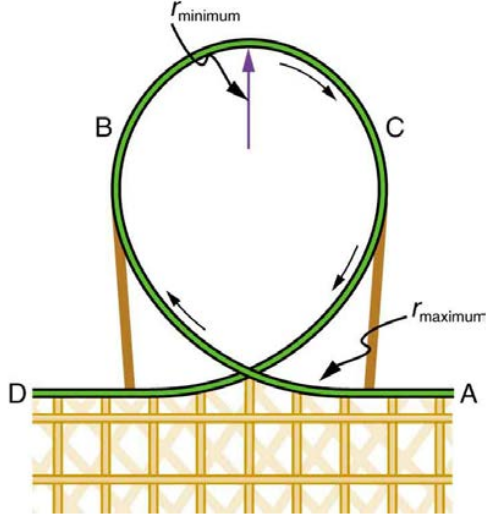
\includegraphics[width=0.4\textwidth]{figures/roll.png}
\end{frame}

\begin{frame}{Examples from Chapter 6}
\small
\textbf{Exercise 31.} \alert{Answer:} We need to consider that the \textit{net force} is the passenger's weight plus centripetal force: $ma = -mg-mv^2/r$.  The minus signs indicate that the the direction of these forces at the top of the loop are \textit{downwards.}  Dividing through by $m$ gives $a=-g-v^2/r$.  We are told that $a/g = -1.5 = -\frac{3}{2}$.  Thus,
\begin{equation}
v = \sqrt{\frac{rg}{2}} = \sqrt{15*10/2} \approx 8.7 ~ m/s
\end{equation}
\end{frame}

\end{document}
